\documentclass[book.tex]{subfiles}
\begin{document}
Wolfenstein layed out the fundation of first person shooter and established id Software as a major development studio. The team embraced their success:\\
\\
Episode 1: Escape from Wolfenstein\\
Episode 2: Operation: Eisenfaust\\
Episode 3: Die, Fuhrer, Die!\\
Episode 4: A Dark Secret\\
Episode 5: Trail of the Madman\\
Episode 6: Confrontation\\

\section{Spears of Destiny}
Released on September 18, 1992 Spears Of Destiny used the same game engine but with new graphics, music and levels. It is a prequel to the adventures of wolf hero: B.J. Blazkowicz \\
   \par
\begin{figure}[H]
\centering
 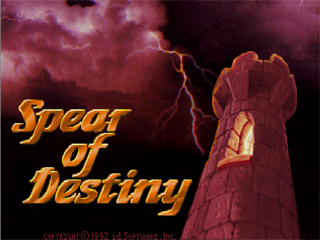
\includegraphics[width=\textwidth]{imgs/spears_of_destiny_intro.png}
 \end{figure}
 \par
 The game resued Wolfenstein3D, allowing a part of the team to release a second title while an other part of the team worked on the next technology to power DOOM. The title was nonetheless innovative (e.g: using transparent sprites to simulate vegetation):
    \par
\begin{figure}[H]
\centering
 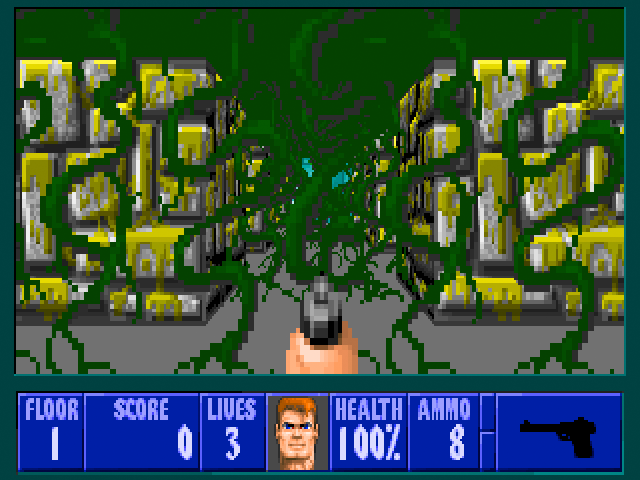
\includegraphics[width=\textwidth]{imgs/spears_of_destiny_play.png}
 \end{figure}
 \par
 SOD features a copy protection mechanism: A set of random question which could only be answered with the game manual:\\
    \par
\begin{figure}[H]
\centering
 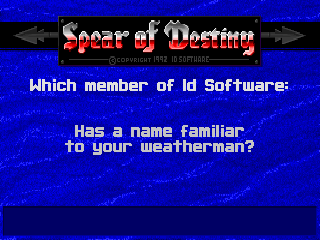
\includegraphics[width=\textwidth]{imgs/spears_of_destiny_copy_protection.png}
 \end{figure}
 \par
 An easter egg is hidden here. A serie of word are always a valid answer. Amond them "Joshua", a reference to 1983 movie WarGames:\\
    \par
\begin{figure}[H]
\centering
 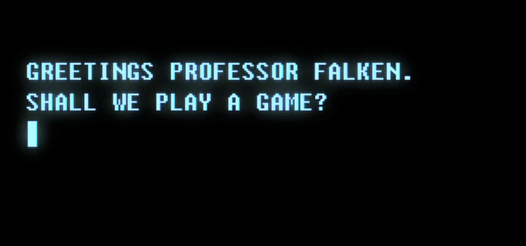
\includegraphics[width=\textwidth]{imgs/spears_of_destiny_easter_egg.png}
 \end{figure}
 \par






It was essentially a mod of Wolfenstein 3D. SOD helps to put things into perspective when it comes to being open source and allow people to figure out the file formats. SOD may not have sold as well had the game been open.\\
No a shareware version  but  2-level playable demo was distributed\\
Lost Episodes, Each of these, consists of 21 levels. New level textures, new enemies, and new appearances for old enemies. Published by FormGen Corporation in May 1994.''
\\
Mission Packs(released by FormGen Corporation in May 1994, resemble many fan-made mods a.k.a: Lost Episodes):\\
Mission 2: Return to Danger\\
Mission 3: Ultimate Challenge\\
\\
Trivia: Angel of Death looked like a demon and was a good insight into what would come next: Doom.
\section{Mission Pack: Return to Danger}
\section{Mission Pack: Ultimate Challenge}
\section{Port: Super Nintendo}
Story of Doom development: They had to stop working on Doom (see GDC for more details).\\
\\
 \begin{fancyquotes}
    When I ported Wolf to the SNES, the ray casting performance cost was too much, so I had to make a new wall span renderer.  Learning about BSP trees allowed me  to much more accurately resolve the culling challenges, and it worked out ok, leading the way to the Doom renderer.\\
\\
Many years later, I made a very similar programming tradeoff for the mobile BREW version of Doom RPG.  The J2ME (java) Doom RPG looked like Wolfenstein, with a tile map world, textured walls, and solid color floor and ceiling, but it was done with a quite nice wall span renderer.  I had learned a thing or two since writing Wolf.  For the ARM native code BREW version, I wanted to add texture mapped floors and ceilings with per-tile texture choices.  I turned the tile maps into polygon windings and started writing a full texture mapped clipped polygon rasterizer for them, but I only had a couple days to work on the mobile renderer, and it became clear that I wasn’t going to be able to deliver a really solid implementation in that time.\\
 \\
The solution was to sacrifice performance for implementation simplicity.  Instead of trying to fill in just the empty pixels around the walls with floor / ceiling textures, I completely textured the entire screen with floor and ceiling textures before drawing the walls on top of them.  With floor / ceiling symmetry and fixed texture sizes, it was pretty fast even with per-pixel tile map lookup, but most importantly it was rock solid, crack free, and completed in the window of time I had allotted to it.\\
\\
\textbf{John Carmack - Programmer}
\end{fancyquotes}
\section{Port: Jaguar}
The jaguar port was release in 1994, it was the only port able to reach 60 frames per seconds. It was unique for having graphics in a resolution much superior to the PC release, and bilinear filtering. It also introduced two new weapons: the Flamethrower and Rocket Launcher:\\


\par

The console was a mix of powerful components with severe bottleneck: 

\begin{fancyquotes}
The memory, bus, blitter and video processor were 64 bits wide, but the processors (68k and two custom risc processors) were 32 bit.\\
\\
The bliter could do basic texture mapping of horizontal and vertical spans, but because there wasn't any caching involved, every pixel caused two ram page misses and only used 1/4 of the 64 bit bus. Two 64 bit buffers would have easily tripled texture mapping performance. Unfortunate.\\
\\
It could make better use of the 64 bit bus with Z buffered, shaded triangles, but that didn't make for compelling games.\\
\\
It offered a usefull color space option that allowed you to do lighting effects based on a single channel, instead of RGB.\\
\\
The video compositing engine was the most innovative part of the console. All of the characters in Wolf3D were done with just the back end scalar instead of bliting. Still, the experience with the limitations and hard failure cases of that gave me good ammunition to rail against microsoft's (thankfully aborted) talisman project.\\
\\
The little risc engined were decent processors. I was surprised that they didn't use off the shelf designs, but they basically worked ok. They had some design hazards (write after write) that didn't get fixed, but the only thing truly wrong with them was that they had scratchpad memory instead of caches, and couldn't execute code from main memory. I had to chunk the DOOM renderer into nine sequentially loaded overlays to get it working (with hindsight, I would have done it differently in about three...).\\
\\
The 68k was slow. This was the primary problem of the system. You options were either taking it easy, running everything on the 68k, and going slow, or sweating over lots of overlayed parallel asm chunks to make something go fast on the risc processors.\\
\\
That is why playstation kicked so much ass for development -- it was programmed like a single serial processor with a single fast accelerator.\\
\\
If the jaguar had dumped the 68k and offered a dynamic cache on the risc processors and had a tiny bit of buffering on the blitter, it could have put up a reasonable fight against sony.\\
\\
\textbf{John Carmack - Programmer (March 4th, 2000)}
\end{fancyquotes}







\section{Port: PC-98}
Essentially Japanese port. Explain the source code diff packages.








\section{Port: 3DO}
Because the 3DO port of Wolfenstein 3D was developed by the same company as the Macintosh port, the two games are nearly identical. They both feature higher resolution graphics, an in-game map, more weapons, and superior audio. However, unlike the original DOS version, the 3DO lacks rotating sprites, so enemies are always looking at you, making it impossible to sneak up on them.






\section{Port: XBox360 and Playstation3}

\begin{fancyquotes}
I also had to make one last minute hack change to the original media — the Red Cross organization had asserted their trademark rights over red crosses (sigh) some time after we released the original Wolfenstein 3D game, and all new game releases must not use red crosses on white backgrounds as health symbols.  One single, solitary sprite graphic got modified for this release.
\\
\textbf{John Carmack - Programmer (Mar 04, 2000)}
\end{fancyquotes}
\section{Port: Macintosh}

Published with authorization

Unlike newer games (Doom, Unreal, etc) the Macintosh version is not just a port (exact translation) of the PC version. The levels and the game engines are actually quite different. Thus, you can not use levels and mods for one version with the other version.\\
\\
\subsection{Levels}

The first major difference is the level design. While the PC version contains 6 episodes with each episode containing 10 levels (1 of those is a hidden bonus level), the Macintosh version (reffered to as the 2nd Encounter) contains 30 levels with no divisions into episodes. The Mac version is divided into floors, but you can not start on a specific floor and every floor has a different amount of levels. A 3rd Encounter was later released for Macintosh containing 60 more levels which were supposed to make up episodes 2 to 6.\\
Obviously, the number of levels aren't the same but this doesn't necessarily mean that the Macintosh version is giving you more. Many of the levels are similar, but the Macintosh levels are usually much less intricate and much shorter. This is apparent in the first level where the path to the exit is exacly the same in both versions, but the PC version contains many more possible side-trips and many more rooms. Other levels in the games are completely different. Basically, the 2 games play extremely differently and offer unique experiences.

\subsection{Game Engine}
Another major difference is in the game engines. At first glance, the Macintosh engine, which is 2 years newer, seems to be the more advanced. The graphics in the Macintosh version are much sharper, clearer, and better looking at twice the resolution of the PC graphics. Also, the game takes up a slightly larger portion of the screen and the sounds are much higher quality in the Macintosh version.\\
However, the enemies in the Macintosh version are only 2D sprites whereas the enemies in the PC version are 3D sprites. This means that the Macintosh enemies only have 1 side, a front side, and thus, they are always facing you. In contrast, the PC enemies have 8 sides, making for much more realist play; in the PC version, it is possible to sneak up behind guards and kill them before they see you - something that can't be done in the Macintosh version.\\
\\
The enemies in the PC version also offer an extra level of realism by being able to patrol an area. In the Macintosh version, the enemies will just stand in one spot until they see you or hear you; in the PC version, enemies will stand in place or patrol an area until they see or hear you. These differences make the PC version's game engine more advanced despite being 2 years older.\\

\subsection{Weapons, Items, and Enemies}

Several other difference worth noting include the addition of 2 extra weapons in the Macintosh version: the flamethrower and the rocket launcher. Those two weapons and some other items (bullet crates, flame thrower and rocket ammo, backpacks) are not found in the PC version.
Also, some other pick-ups and dropped items are different. For example, in the PC version, dropped clips give 4 ammo and other clips give 8 ammo; in the Macintosh version, all clips give 5 ammo. Also, picking up treasure in the PC version adds to your score (40000 points gets you an extra life); in the Macintosh version, picking up treasure increases your item count by one until you get an extra life at 50 items.

Other differences include an additional enemy, the Flying Hitler, in the PC version and different bosses in the 2 versions (see the enemies and bosses pages); the Mac version actually uses some bosses from Wolfenstein 3D and some bosses from Spear of Destiny.

\subsection{Miscellaneous}

Yet another difference is that changing the difficulty level in the Macintosh version only affects the damage taken and starting ammo whereas in the PC version it affects the damage taken and the number of enemies; the PC version tends to be much more difficult. The Macintosh version also has an auto-map that is helpful in finding you way around; there is no mapping feauture in the PC version.
The last difference I can think of is the pools of blood in the PC version. In the Mac version, you only have pools of water - no pools of blood. If your health is less than 11 in the PC version, you can drink the blood to gain back some health.



\section{Port: Game Boy Advance}
Released in 2002, the Game Boy Advance version is an nearly exact port of the PC version. It contains all 6 Episodes. The only difference is that you can only save the game at the end of a level - not during.

\section{Modding}

\end{document}